% !TEX root = thesis-thomas-tiotto.tex

\section{Methods} 

\subsection{Libraries}\label{subsec:libraries}
\subsubsection{Pomegranate}
\textit{Pomegranate} (\cite{pomegranate}) is an open-source probabilistic models package for Python.
Its core philosophy is that every probabilistic model, from Hidden Markov to Bayesian Network, can be seen as a probability distribution and, as such, can be flexibly composed into hierarchical mixture models (\cite{Schreiber2017}).
The package implements:
\begin{itemize}
	\item Probability Distributions
	\item General Mixture Models
	\item Hidden Markov Models
	\item Bayes Classifiers and Na{\"i}ve Bayes
	\item Markov Chains
	\item \textbf{Bayesian Networks}
	\item Factor Graphs
\end{itemize} 

This package was chosen among others for its good implementation of Bayesian Networks and its performance.
The package is written in cython and natively supports multi-core parallelism and out-of-core learning.
Network structure learning from data, described in \ref{subsec:bnstructurelearning}, appears to be particularly efficient, thanks to the implementation of prior knowledge into the graph selection process as described by \cite{schreiber_noble_2017}.
The claim of this novel selection process is that it possesses the speed of a heuristic approach while yielding a far better quality estimate.

Pomegranate currently only supports Discrete Bayesian Networks so the random variable of each node must have a categorical distribution.

\textit{Structure learning} from data is achieved using the \texttt{from\_samples} method of the \texttt{BayesianNetwork} class, with the default algorithm being the novel one described by \cite{schreiber_noble_2017}.
The \textit{probability} of a sample is calculated using the \texttt{probability} function of an object of \texttt{BayesianNetwork} type; the \texttt{predict\_proba} function is used to return the probability of each variable in the model given some evidence.
\textit{Predictions} (described in detail in Subsec. \ref{subsec:bnupdating}) are run by passing to the \texttt{predict} function of an object a matrix with \texttt{None} as placeholders for missing values .
\textit{Fitting} is done thought the \texttt{fit} function that uses MLE estimates to update each node's distribution in the model based on the input data.

A \texttt{BayesianNetwork} object can also be displayed graphically by calling its \texttt{plot} function.
The output is a DOT file that is generated using the PyGraphviz package (\cite{pygraphviz}), that is a python interface to the famous Graphviz (\cite{graphviz}) graph visualisation software.
An example of such an output is shown in Fig. \ref{fig:pomegranate_graph_example}.

\begin{figure}[htbp]
\centerline{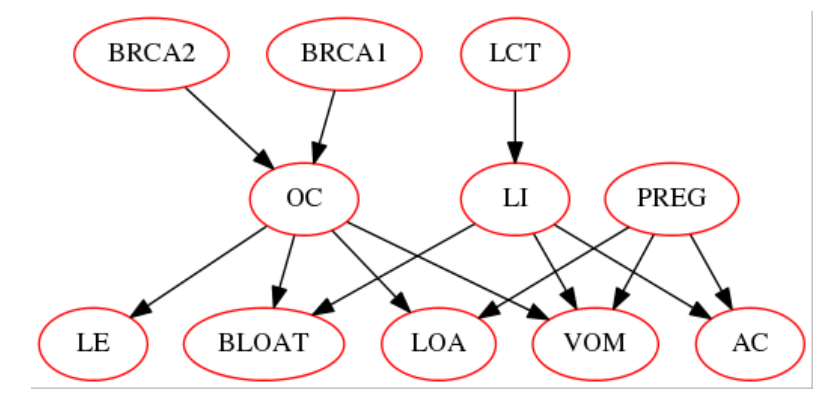
\includegraphics[width=\columnwidth]{methodology/images/pomegranate_example}}
\caption{Example output of \texttt{plot} (\cite{pomegranatetutorial}) }
\label{fig:pomegranate_graph_example}
\end{figure}

\subsubsection{Pgmpy}
\textit{Pgmpy} (\cite{pgmpy}) is, like pomegranate, another recent probabilistic graphical model package for Python.
Unlike pomegranate, it natively implements various exact and approximate inference algorithms, like Variable Elimination, Belief Propagation and Max-Product Linear Programming.

The reason that I elected to use two different probabilistic graphical model libraries is because there is still no Python package that offers all the needed functionality.
Pomegranate implements a novel structure learning algorithm, that I wanted to use, but is severely lacking in functionality in many other areas.
Pgmpy, on the other hand, has a very good API as regards inference.

\subsubsection{DAOOPT}
\textit{DAOOPT} is an open-source implementation of sequential AND/OR Branch-and-Bound proposed by \cite{Marinescu2006}.
Search-based algorithms traverse the model's search space and are much more efficient in their use of space, compared to inference-based algorithms such as Variable Elimination.

DAOOPT builds an AND/OR search space to generate search an AND/OR graph that takes advantage of information encoded in the graphical model, namely its independencies.
The DAOOPT implementation found at \cite{daoopt} is an exact solver for finding an MPE solution in Bayesian Networks.
The solver is written in C++ and accessible through a command-line interface; the only required parameter is a \texttt{.uai} file representing a Markov Random Field or a Bayesian Network but in most cases an optional \texttt{.uai.evid} file will also be given, containing the observed evidences.

\subsubsection{UAI file format}
The \texttt{.uai} file format is a simple text file used to represent problem instances.
Such a file is composed of:
\begin{itemize}
  \item Preamble: containing the type of the network (MARKOV or BAYES), the number and cardinality of variables and the cliques, that in the BAYES case are simply the variables appearing in each Conditional Probability Table (CPT) 
  \item Function tables: containing the actual definition of the CPTs i.e. the values of each node give its parents or, in the case of root nodes, the marginal probabilities.
\end{itemize}

The \texttt{.uai.evid} is a very simple file containing the number of variables in the evidence set followed by the index of each variable and its observed value.
In both formats the variables and their values are represented only by a numerical index, starting from $0$, with the ordering being defined in the preamble of the \texttt{.uai} and maintained consistent throughout the \texttt{.uai} and \texttt{.uai.evid}.

Following, is the \texttt{.uai} representing the network shown in Fig. \ref{fig:bn-example-dag}, that has been our running example throughout the last chapters.
Lines starting with \texttt{c} are interpreted as comments; these are misinterpreted by DAOOPT and are thus removed when running it, but are here shown for clarity.
The file starts by stating that the model is a Bayesian Network composed of 5 random variables that will then be referenced by an ordinal index starting at 0; the first variable (index 0) is of cardinality 3, the second (index 1) is of cardinality 2 and so on.
We can then see the definition of the cliques or more precisely, as our model is a BN and not a MRF, of the CPTs; there are 5 of these, each one associated to one of the five variables just stated.
The first CPT involves 2 random variables: the first (0) and the second (1); the second CPT involves only one variable (1) and this tells us that variable 1 is a root node in the BN's DAG.
The ordering is such that the child node is the last in the definition of each CPT's nodes so, for example, in the first CPT we find that variable 1 is the child of variable 0.
Finally, we have a complete definition of the function tables/CPTs.
The tables are printed so that each row corresponds to the conditional probability value of the child node and increasing rows correspond to increasing enumeration of the parents' states, in the order given when defining the variables involved in the CPTs.
The first table corresponds to \textbf{eta arrotondata}'s CPT shown in Tab. \ref{tab:eta-cpd}.
It contains 6 elements as it involves variables 0 (\textbf{mut17q21}) and 1 (\textbf{eta arrotondata)} that are of cardinality 2 and 3, respectively.
So each row corresponds to the probability distribution of the three states of variable 1, given each of the two states of variable 0.

\begin{verbatim}
c
c Bayesian Network exported from pomegranate - Thomas Tiotto (2019)
c

BAYES
5
3 2 3 3 2 

c
c Cliques
c

5
2 0 1 
1 1 
2 2 1 
3 3 2 4 
1 4 

c
c CPTs
c

6
 0.42105263157894735 0.42105263157894735 0.15789473684210523 
 0.043798177995795384 0.17063770147161877 0.7855641205325858 

2
 0.006613296206056387 0.9933867037939436 

6
 0.6842105263157895 0.0 0.3157894736842105 
 0.1373510861948143 0.021723896285914507 0.8409250175192712 

18
 0.004385964912280701 0.2412280701754386 0.7543859649122807 
 0.022598870056497175 0.11864406779661016 0.8587570621468926 
 0.10344827586206899 0.41379310344827586 0.4827586206896552 
 0.2121212121212121 0.45454545454545453 0.3333333333333333 
 0.14094488188976378 0.6362204724409449 0.22283464566929131 
 0.289612676056338 0.5677816901408451 0.1426056338028169 

2
 0.5315001740341107 0.4684998259658893 
\end{verbatim}

The following is an example of a randomly generated \texttt{.uai.evid} evidence file that simply states that the evidence set has cardinality 2 and contains variable 4 (in the ordering given in the \texttt{.uai}) in its state 1 and variable 3 in state 2.

\begin{verbatim}
 2
  4 1
  3 2
\end{verbatim}

These were generated by a function I have written (see \ref{subsec:algorithms}) that is able to export a \texttt{pomegranate} model and randomly generated evidence to the correct imput format for DAOOPT.

\subsubsection{Gurobi}
\textit{Gurobi} (\cite{gurobi}) is a closed-source mathematical programming solver for Linear Programming, Quadratic Programming and Mixed-Integer Programming optimisation problems.
It claims to be the fastest solver available for these classes of problems.
Gurobi offers object-oriented and matrix-oriented interfaces to, among others, Python, MATLAB and Excel.

\subsubsection{Pandas}
\textit{pandas} (\cite{pandas}) is an extremely widely-used open-source python library that provides data structures and methods to aid in data analysis.
The package excels in the manipulation of tabular data in the form of \texttt{DataFrame}, that is the analogous of R's \texttt{data.frame}.
A \texttt{DataFrame} can be seen as a \enquote{general 2D, size-mutable structure with potentially heterogeneously-typed columns}.
The syntax for slicing is very close to R's as are many other functionalities; this is because one of Pandas' explicit goals is to offer all of CRAN's functionalities and be easily approachable by anyone already knowing the other language.

Pandas the default choice for this thesis' implementation because it is the \textit{de facto} standard in data analysis applications.
Its flexibility in reading Excel spreadsheets (the format the data set the project was built on, see Sec. \ref{sec:data-set}) and in then manipulating the data confirmed that this was a good choice.
Note that to read files in the Excel formats the additional \texttt{xlrd} package is needed.

\subsubsection{Scikit-learn}
\textit{scikit-learn} (\cite{scikitlearn}) aims at providing a unified API for basic Machine Learning; it does not include advanced paradigms such as Reinforcement Learning or graphical models for structured learning.
The latter omission was the reason that lead me to select pomegranate as the basis for the implementation of a Bayesian Network.
What is included are a stack supervised and unsupervised ML tools to prepare data sets, define machine learning models ranging from spectral analysis-based to ensemble methods to clustering and multiple evaluation and model selection utilities.

\subsubsection{NumPy}
\textit{NumPy} (\cite{numpy}) is another \textit{de facto} standard package when doing scientific computing with python.
Most scientific packages (including pandas, scikit-learn and TensorFlow) depend on NumPy for low-level operations; this is because NumPy is contains fast implementation of n-dimensional array objects together with powerful manipulation functions.
In addition to this, NumPy implements linear algebra operations, Fourier Transform and random number generation.
The closest parallel to NumPy - as R was for pandas, is MATLAB.

\subsubsection{Networkx}
\textit{NetworkX} (\cite{networkx}) is another widely-used package that is specialised in the creation and manipulation of graph-structured data.
The main use for this package was in building the \texttt{MPEGraph} data structure that I used to build a polytree representing the dialogue with the expert.

\subsection{Algorithms} \label{subsec:algorithms}
\todo{quanti dettagli implementativi devo mettere?  perchè ho un sacco di funzioni di visualizzazione etc}

\subsubsection{Model construction}
The data was given in \texttt{.xlsx} format and was imported using \texttt{panda}'s \texttt{read\_excel} function that returned a \texttt{DataFrame} object.
The imported data was then preprocessed by dropping unwanted records and binning the remaining ones as described in Tab. \ref{tab:datasetpreprocess} .
The actual BN representation is learned at runtime by calling the \texttt{from\_samples} method of \texttt{pomegranate}'s \texttt{BayesianNetwork} to solve the structure learning problem (defined in Subsec. \ref{subsec:bnstructurelearning}).

The binned data was codified into integer representations before being passed to pomegranate's structure learning algorithm.
Thus the network's state names are in natural language but the internal representation of the values of each random variable is an integer number.
A dictionary object is used to translate one representation into the other at runtime.

\subsubsection{d-separation}
A na{\"i}ve implementation according to the definition (presented in Subsec. \ref{subsec:d-separation}) to check for d-separation between node $X$ and $Y$ would have a complexity in the order of the number of trails between $X$ and $Y$; this would lead to an exponential in the size of the graph running time.
Luckily, \cite{koller2007dseparation} present a linear time algorithm to solve the problem.

The \texttt{reachable} procedure takes as input the DAG representing the Bayesian Network $\mathcal{G}$, a source variable $X$ and a set of observed variables $Z$; on exit it returns the set of variables $R$ that are reachable from $X$.
The procedure runs in two phases, traversing the graph twice: first bottom-up from leaves to roots, then viceversa.
During the first run, the algorithm finds all nodes $A$ that are ancestors of the evidence set $Z$.
During the second, the procedure distinguishes the direction it visits each node in order to determine if it is traversable or not.
Any node $Y$ that is not in the evidence set is marked as reachable; if it is being visited in direction \enquote{up} it can be traversed as the v-structure is a chain.
All the parents of $Y$ are marked to be visited in the \enquote{up} direction (i.e. from below) and the converse is done for $Y$'s children.
If $Y$ is being visited in the \enquote{down} direction its children are again added to be visited in the \enquote{down} direction, because $Y$ is traversable.
Additionally, if $Y$ happened to be in the set $A$, found in the first step, then $Y$'s parents are marked to be visited in the \enquote{up} direction because the collider is active and $Y$ can be traversed (a collider is open iff. the central node or any of its descendants are observed).

The full procedure can be found in \cite{koller2007dseparation}; my implementation follows this pseudocode very closely but the procedure \texttt{d-separated}, instead of finding all nodes $R$ that are d-connected to the input $X$, tests if a given target $Y$ is d-separated from $X$ or not, as is shown in Alg. \ref{alg:d-separation}.
This gives some extra flexibility in how the function can be used.
To find the set $S$ of all nodes d-separated from $X$ I simply iterate the \texttt{d-separated} test over all nodes $V$ in the graph representing the BN.

\begin{algorithm}[htp!]
	\caption{d-separation algorithm}
	\label{alg:d-separation}
	\begin{algorithmic}[1]
		\State $separated\_list = \emptyset$
		\For{target $Y \in V$} 
			\State append $d-separated(X, Y, E)$ to $separated\_list$ \Comment{will return true or false}
		\EndFor
	\end{algorithmic}
\end{algorithm}

\subsubsection{MPE}
The solution to the Most Probable Explanation problem (MPE), as defined in Subsec. \ref{subsec:bnupdating}, is found by using DAOOPT (Subsec. \ref{subsec:libraries} ) as an external solver.
The latest version of DAOOPT was downloaded from the github page (\cite{daoopt}) and compiled into a executable.
DAOOPT only offers a command line interface so some extra work was needed in order to interface it with the Python-based application I have developed.
The connection was done by first writing to stable storage a \texttt{.uai} containing the model definition and a \texttt{.uai.evid} with the observed evidence.
These files are then piped to DAOOPT by using Python's \texttt{subprocess} module to run the following command in an external background shell:
\begin{verbatim}
	./daoopt -f pomegranate.uai -e pomegranate.uai.evid
\end{verbatim}
The shell output is captured and also written to stable storage, in order to be decoded and used in the system.

To exemplify the process, we return to the example used while presenting DAOOPT in Subsec. \ref{subsec:libraries}.
Given the \texttt{.uai} representing the BN and the \texttt{.uai.evid} random evidence:
\begin{verbatim}
 2
  4 1
  3 2
\end{verbatim}
DAOOPT would give the following output:
\begin{verbatim}
	--- Starting search ---
[0] u 3 4 -1.3581 5 2 1 2 2 1
[0] Cache statistics: . . . .

--------- Search done ---------
Problem name:  pomegranate
OR nodes:      3
AND nodes:     4
OR processed:  3
AND processed: 8
Leaf nodes:    2
Pruned nodes:  4
Deadend nodes: 1
Time elapsed:  0 seconds
Preprocessing: 0 seconds
-------------------------------
-1.3581 (0.0438433)

p 2 1 2
l 2 1 6
s -1.3581 5 2 1 2 2 1
\end{verbatim}
The end of the final line is the one of interest as it is the assignment of values to the variables that solves the MPE problem.
The \texttt{5 2 1 2 2 1} string is to be interpreted as meaning:
\begin{itemize}
  \item there are 5 variables in the solution
  \item the variable indexed by 0 (in the ordering given in the preable of the \texttt{.uai}) is assigned its second value (the ordering is inferred by the CPTs defined in the \texttt{.uai}) in the MPE solution
  \item variable 1 is assigned its second value
  \item variable 2 is assigned its third value
  \item variable 3 is assigned its third value
  \item variable 4 is assigned its second value
\end{itemize}
Variables 3 and 4 are constrained to assume the value specified in the input \texttt{.uai.evid}; in this case 1 and 2, respectively.

All the functionality relating to solving the MPE with DAOOPT is encapsulated in the \texttt{daoopt\_solver} function that given the input \texttt{.uai} files, returns the MPE solution.

\subsubsection{Other Machine Learning methods}
In order to quantify the prediction capabilities of the Bayesian Network, that is at the heart of this thesis' methods, I implemented a series of tests to find the best performing algorithm on the data set.
Given that the performance of Machine Learning algorithms is heavily dependent on the input classes, I used a process of \textit{exhaustive variable elimination} in order to identify the most relevant features for the predictions.
In parallel, I scored each input subset using the following ML algorithms, in order to find the best performing one:
\begin{itemize}
  \item Linear Regression: this method assumes that the relationship between the dependent variable $y$ and the regressors $x$ is linear i.e. that $y$ can be written as a linear combination of $x$'s components: $y = \beta_0 + \beta_1 x_1 + \ldots \beta_n x_n$.
  \item Logistic Regression: is used in lieu of Linear Regression when the values of the variables are categorical; it assumes that the relationship between the regressors $x$ and the log-odds of $y$ are linear i.e. $\log _{b} \frac{p}{1-p}=\beta_{0}+\beta_{1} x_{1}+ \ldots + \beta_{n} x_{n}$ with $p$ the probability of the event of interest.
  \item Linear Discriminant Analysis: LDA is related to Principal Component Analysis (PCA) in that it attempts to find a linear equation modelling the data but LDA explicitly tries to express the difference between the data classes.
  \item Decision Tree: a Decision Tree is built using a recursive, greedy algorithm that continually splits the dataset into two.  The variable along which to bisect is the one that yields the lowest accuracy loss in the resulting split.
  \item Na{\"i}ve Bayes: a Na{\"i}ve Bayes classifier is a conditional probability model that given features $x_1 \ldots x_n$, attempts to assign a probability to each of the possible outcomes $O_{k}$ of interest by using Bayes' Theorem (Eq. \ref{eq:bayes-theorem} ): $\mathbb{P}\left(O_{k} | x \right)=\frac{\mathbb{P}\left(O_{k}\right) \mathbb{P}\left(x| O_{k}\right)}{\mathbb{P}(x)}$.  The method is called \enquote{na{\"i}ve} because of a strong (ofter unrealistic) assumption of all the features $x_1 \ldots x_n$ being independent.
  \item K-Nearest Neighbours: the algorithm is non-parametric with the output class depending on the predominant class among the $k$ nearest neighbours (according to some distance metric) of the input vector $x$.
  \item Support-Vector: A Support-Vector Machine (SVM) is an algorithm that attempts to find the set of \textit{best-separating hyperplane} between classes of objects, seen as points in a high-dimensional space.  Such a hyperplane is the one that has maximum distance from the closest representatives of each class.
  \item Random Forest: this is an ensemble method that aims to correct Decision Trees' tendency to overfit the data.  A multitude of Decision Trees is constructed and the final classification output is the class that appears most often in the intermediate step.
  \item AdaBoost: Short for \textit{Adaptive Boosting}; this meta-learning, ensemble algorithm combines a series of weak classifiers, that may only be slight better than a random guess, through a weighted sum into a \textit{strong classifier}.  It is a meta-learning algorithm because the weak classifiers are revised over a series of iterations in order to improve their performance on previously misclassified instances.
  \end{itemize}



